\documentclass[12pt,a4paper]{article}



\usepackage[utf8]{inputenc}
\usepackage{amsmath}
\usepackage{amsfonts}
\usepackage{amssymb}
\usepackage{graphicx}
\usepackage{amsthm}
\usepackage{natbib}
\usepackage{algorithm}
\usepackage{algpseudocode}

\usepackage{hyperref}
\AtBeginDocument{\let\textlabel\label}

\usepackage{marginnote}
\renewcommand*{\marginfont}{\footnotesize}







\theoremstyle{plain}
\newtheorem{thm}{Theorem}
\newtheorem{lemma}{Lemma}
\newtheorem{prop}{Proposition}

\theoremstyle{definition}
\newtheorem{definition}{Definition}
\newtheorem{remark}{Remark}
\newtheorem{example}{Example}


\newcommand{\naive}{na\"{\i}ve }
\newcommand{\Naive}{Na\"{\i}ve }

\newcommand{\expect}[1]{E\left[ #1 \right]}
\newcommand{\expectg}[2]{E_{#1}\left[ #2 \right]}
\newcommand{\expectn}[1]{\mathbb{E}\left[#1\right]}
\newcommand{\gauss}[1]{\mathcal{N}\left(#1\right)}
\newcommand{\cdf}{F}
\newcommand{\cdfn}{\mathbb{F}}
\newcommand{\icdf}{F^{-1}}
\newcommand{\icdfn}{\mathbb{F}^{-1}}
\newcommand{\pdf}{p}
\newcommand{\dist}{P}

\newcommand{\norm}[1]{\Vert #1 \Vert}
\newcommand{\lik}{\mathcal{L}}
\newcommand{\loglik}{L}
\newcommand{\loss}{l}
\newcommand{\risk}{R}
\newcommand{\riskn}{\mathbb{R}}
\newcommand{\deriv}[2]{\frac{\partial #1}{\partial #2}}
\newcommand{\argmin}[2]{argmin_{#1}\left\{ #2 \right\}}
\newcommand{\hyp}{f}
\newcommand{\hypclass}{\mathcal{F}}
\newcommand{\plane}{\mathbb{L}}
\newcommand{\categories}{\mathcal{G}}
\newcommand{\positive}[1]{\left[ #1 \right]_+}
\newcommand{\kernel}{\mathcal{K}}
\newcommand{\featureS}{\mathcal{X}}
\newcommand{\indicator}[1]{I_{\{ #1 \}}}
\newcommand{\similarity}{d}






\newcommand{\sample}{\mathcal{S}}
\newcommand{\test}{\risk(\hyp)}
\newcommand{\train}{\riskn(\hyp)}
\newcommand{\insample}{\bar{\risk}(\hyp)}
\newcommand{\EPE}{\risk(\hat{\hyp}_n)}
\newcommand{\folds}{K} % Cross validation folds
\newcommand{\fold}{k}
\newcommand{\bootstraps}{B} % Bootstrap samples
\newcommand{\bootstrap}{{b^*}}




\author{Jonathan Rosenblatt}
\title{Class Notes (experimental)}




\begin{document}

\maketitle

This text draws from \cite{hastie_elements_2003} and \cite{shalev-shwartz_understanding_2014}.
The former is freely available online.
For a softer introduction, with more hands-on examples, see \cite{james_introduction_2013}, also freely available online.
All books are very well written and strongly recommended.


\tableofcontents


\section{Estimation}
\label{sec:estimation} 
In this section, we present several estimation principeles. 
Their properties are not discussed, as the section is merely a reminder and a preparation for what follows.
These concepts and examples can be found in many introductory books to statistics. I particularly recommend \cite{wasserman_all_2004} or \cite{abramovich_statistical_2013}.

\subsection{Moment matching}
\label{sec:moment_matching}

The fundamental idea: match empirical moments to theoretical. I.e., estimate
$$ \expect{g(X)}   $$
by 
$$ \expectn{g(X)}   $$
where $\expectn{g(X)}:=\frac{1}{n}  \sum_i g(X_i)$, is the empirical mean.

\begin{example}[Exponential Rate]

Estimate $\lambda$ in $X_i \sim exp(\lambda)$, $i=1,\dots,n$, i.i.d.
$\expect{X}=1/\lambda$.
$\Rightarrow \hat{\lambda}=1/\expectn{X}$ 

\end{example}


\begin{example}[Linear Regression]

Estimate $\beta$ in $Y \sim \gauss{X\beta,\sigma^2 I}$, a $p$ dimensional random vector.
$\expect{Y}=X\beta$ and $\expectn{Y}=y$.
Clearly, moment mathing won't work because no $\beta$ satistifes $X\beta=Y$.
A technical workaround:
Since $\beta$ is $p$ dimensional, I need to find some $g(Y): \mathbb{R}^n \mapsto \mathbb{R}^p$.
Well, $g(Y):=XY$ is such a mapping. I will use it, even though my technical justification is currently unsatisfactory. We thus have:
$\expect{X'Y}=X'X\beta$ which I match to $\expectn{X'Y}=X'y$:
$$
  X'X \beta = X' y \Rightarrow \hat{\beta}=(X'X)^{-1} X'y.
$$

\end{example}


\subsection{Quantile matching}
\label{sec:quantiles}
The fundamental idea: match empirical quantiles to theoretical. 
Denoting by $\cdf_X(t)$ the CDF of $X$, then $\icdf_X(\alpha)$ is the $\alpha$ quantile of $X$.
Also denoting by $\cdfn_X(t)$ the Empirical CDF of $X_1,\dots, X_n$, then $\icdfn_X(\alpha)$ is the $\alpha$ quantile of $X_1,\dots, X_n$.
The quantile matching method thus implies estimating
$$ \icdf_X(\alpha)   $$
by 
$$ \icdfn_X(\alpha)  . $$

\begin{example}[Exponential rate]
Estimate $\lambda$ in $X_i \sim exp(\lambda)$, $i=1,\dots,n$, i.i.d.
\begin{align*}
	& \cdf_X(t) = 1-\exp(-\lambda t) = \alpha \Rightarrow \\
	& \icdf_X(\alpha) = \frac{-\log(1-\alpha)}{\lambda} \Rightarrow \\
	& \icdf{X}{0.5} = \frac{-\log(0.5)}{\lambda} \Rightarrow \\
	& \hat{\lambda} = \frac{-\log(0.5)}{\icdfn{X}{0.5}}.
\end{align*}

\end{example}


\subsection{Maximum Likelihood}
\label{sec:ml}

The fundamental idea is that if the data generating process (i.e., the \emph{sampling distribution}) can be assumed, then the observations are probably some high probability instance of this process, and not a low probability event:
Let $X_1,\dots,X_n \sim P_\theta$, with density (or probability) $p_\theta(X_1,\dots,X_n)$.
Denote the likelihood, as a function of $\theta$: $\lik(\theta): p_\theta(X_1,\dots,X_n)$.
Then $$\hat{\theta}_{ML}:= argmax_{\theta}\{ \lik(\theta) \}$$.

Using a monotone mapping such as the log, does not change the $argmax$. 
Denote $$\loglik(\theta):=\log(\lik(\theta))$$.

 
\begin{example}[Exponential rate]

Estimate $\lambda$ in $X_i \sim exp(\lambda)$, $i=1,\dots,n$, i.i.d.
Using the exponential PDF and the i.i.d. assumption
$$ \lik(\lambda) = \lambda^n \exp(-\lambda \sum_i X_i), $$
and 
$$ \loglik(\lambda) = n \log(\lambda) -\lambda \sum_i X_i. $$

By differentiating and equating $0$, we get $\hat{\lambda}_{ML}=1/\expectn{X}$.

\end{example}

\begin{example}[Discrete time Markov Chain]

Estimate the transition probabilities,  $p_1$ and $p_2$ in a two state, $\{0,1\}$, discrete time, Markov chain where:
$P(X_{t+1}=1|X_{t}=0)=p_1$ and $P(X_{t+1}=1|X_{t}=1)=p_2$.
The likelihood:
$$
  \lik(p_1,p_2)=
  P(X_2,\dots,X_T;X_1,p_1,p_2)=
  \prod_{t=1}^T P(X_{t+1}=x_{t+1}|X_{t}=x_t).
$$
We denote $n_{ij}$ the total number of observed transitions from $i$ to $j$ and get that $\hat{p}_1=\frac{n_{01}}{n_{01}+n_{00}}$, and that $\hat{p}_2=\frac{n_{11}}{n_{11}+n_{10}}$.

\begin{remark}
Well, this is a rather artificial example, as because of the Markov property, and the stationarity of the process, we only need to look at transition events, themselves Brenoulli distributed. 
This example does show, however, the power of the ML method to deal with non i.i.d. samples. As does the next example.
\end{remark}
\end{example}

\begin{example}[Brownian motion with drift]
Estimate the drift parameter $a$,  in a discrete time Gaussian process where:
$X_{t+1}=X_t+\varepsilon; \varepsilon \sim \gauss{0,\sigma^2} \Rightarrow X_{t+1}|X_t \sim \gauss{a X_t,\sigma^2}$.

We start with the conditional density at time $t+1$:
$$
  p_{X_{t+1}|X_t=x_t}(x_{t+1}) = 
  (2 \pi \sigma^2)^{-1/2} \exp \left( 
    -\frac{1}{2 \sigma^2}(x_{t+1}-a x_t)^2 
  \right).
$$
Moving to the likelihood:
$$
  \lik(a) = 
  (2 \pi \sigma^2)^{-T/2} \exp \left(
    -\frac{1}{2 \sigma^2}\sum_{t=1}^T (x_{t+1}-a x_t)^2 
  \right).
$$
Differentiating with respect to $a$ and equating $0$ we get $\hat{a}_{ML}=\frac{\sum x_{t+1}x_{t}}{\sum x_t^2}$.

We again see the power of the ML device.
Could we have arrive to this estimator by intuiton alone? Hmmmm... maybe. 
See that $Cov[X_{t+1},X_t] = a \; Var[X_t] \Rightarrow a=\frac{Cov[X_{t+1},X_t]}{Var[X_t]}$.
So $a$ can also be derived using the moment matching method which is probably more intuitive.

\end{example}

\begin{example}[Linear Regression]

Estimate $\beta$ in $Y \sim \gauss{X\beta,\sigma^2 I}$, a $p$ dimensional random vector.
Recalling the multivariate Gaussian PDF:
$$
  p_{\mu,\Sigma}(y) = 
  (2 \pi)^{-n/2} |\Sigma|^{-1/2} \exp\left(
    -\frac{1}{2} (y-\mu)' \Sigma^{-1} (y-\mu)
  \right)
$$
So in the regression setup:
$$
  \lik(\beta)= 
  p_{\beta,\sigma^2}(y) = 
  (2 \pi)^{-n/2} |\sigma^2 I|^{-1/2} \exp\left(
    -\frac{1}{2 \sigma^2} \norm{y-X\beta}^2
  \right)
$$
and $\hat{\beta}_{ML}$ equals 
\begin{align}
	\hat{\beta}_{ML}=(X'X)^{-1} X'y.
\end{align}


\end{example}


\subsection{M-Estimation and Empirical Risk Minimization}
\label{sec:m_estimation}

M-Estimation, know as Empirical Risk Minimizaton (ERM) in the machine learning literature, is a very wide framework which stems from statistical desicion theory.
The underlying idea is that each realization of $X$ incurs some loss, and we seek to find a "policy", in this case a parameter, $\theta^*$ that minimizes the average loss.
In the econometric literature, we dot not incur a loss, but rather a utility, we thus seek a policy that maximizes the average utility.

Define a loss function $\loss(X;\theta)$, and a risk function, being the expected loss, 
$\risk(\theta):=\expect{\loss(X;\theta)}$. Then \marginnote{Risk}
\begin{align}
\label{eq:risk_min}
 \theta^*:= \argmin{\theta}{\risk(\theta)}.
\end{align}



As we do not know the distribution of $X$, we cannot solve Eq.(\ref{eq:risk_min}), so we minimize the \emph{empirical} risk. \marginnote{Empirical Risk}
Define the empirical risk as $\riskn(\theta):=\expectn{\loss(X;\theta)}$, then 
\begin{align}
\label{eq:empirical_risk_min}
 \hat{\theta}:= \argmin{\theta}{\riskn(\theta)}.
\end{align}

\begin{remark}
The risk function, $\risk(\theta)$ defined above
\end{remark}



\begin{example}[Squared Loss]
Let $\loss(X;\theta)=(X-\theta)^2$. Then 
$
	\risk(\theta) = 
	\expect{(X-\theta)^2} = 
	(\expect{X}-\theta)^2 + Var[X]. 
$
Clearly  $Var[X]$ does not depend on $\theta$  so that $\risk(\theta)$ is minimized by $\theta^*=\expect{X}$.
\textbf{We thus say that the expectation of a random variable is the minimizer of the squared loss.}

How do we estimate the population expectation? Well a natural estimator is the empirical mean, which is also the minimizer of the empirical risk $\riskn(X)$. The proof is immediate by differentiating. 
\end{example}


\begin{example}[Least Squares Regression]
\label{eg:OLS}
Define the loss $\loss(Y,X;\beta):=\frac{1}{2}(Y-X\beta)^2$.
Computing the risk, $\expect{\norm{Y-X\beta}^2}$ will require dealing with the $X$'s by either assuming the \emph{Generative Model}\footnote{A Generative Model is a supervised learning problem where the we use the assumed distribution of the $X$s and not only $Y|X$. The latter are know as Discriminative Models.}, as expectation is taken over $X$ and $Y$. \marginnote{Generative Model}
We don't really care about that right now. 
We merely want to see that the empirical risk minimizer, is actually the classical OLS Regression. And well, it is, by definition...
\begin{align*}
	\riskn(\beta)=\sum_{i=1}^n 	\frac{1}{2}(y-x_i\beta)^2 = \frac{1}{2}\norm{y-x\beta}^2.
\end{align*}
Minimization is easiest with vector derivatives, but I will stick to regular derivatives:
\begin{align*}
	\deriv{\riskn(\beta)}{{\beta_j}} = \sum_i \left[ (y_i-\sum_{j=1}^p x_{ij}\beta_j)(-x_{ij}) \right]
\end{align*}
Equating $0$ yields $\hat{\beta_j}=\frac{\sum_i y_i x_{ij}}{\sum_i x_{ij}^2}$.
Solving for all $j$'s and putting in matrix notation we get
\begin{align}
	\hat{\beta}_{OLS}=(X'X)^{-1} X'y.
\end{align}


\end{example}


\subsection{Notes}
\paragraph{Maximum Likelhood} 
If we set the loss function to be the negative log likelihood of the (true) sampling distribution, we see that maximum likelihood estimators in independent samples are actually a certain type of M-estimators.


\section{From Estimation to Supervised Learning}
\label{sec:learning}

\subsection{Empirical Risk Minimization (ERM) and Inductive Bias}
In Supervised Learning, or \emph{learning with teacher} problems where we want to extract the relation $y=\hyp(x)$ between attributes $x$ and some outcome $y$.
It is implicit, and essential, that the outcomes are observed. If this is not the case, see Unsupervised Learning (\S\ref{sec:unsupervised})
The attributes, also know as features, or predictors, are assumed to belong to some \emph{feature space} $\featureS$. \marginnote{Feature Space}

In particular, we don't need to explain the causal process relating the two, so there is no need to commit to a sampling distribution. The implied ERM problem is thus
\begin{align}
	\hat{\hyp}(x) = \argmin{\hyp}{\sum_i \loss(y_i - \hyp(x_i))}.
\end{align}
Alas, there are clearly infinitely many $\hyp$ for which $\riskn(\hat{\hyp}(x))=0$, in particular, all those where $\hat{\hyp}(x_i)=y_i$.
All these $\hyp$ feel like very bad predictors, as they \emph{overfit} the observed data, at a cost of generalizability.\marginnote{Overfitting}
We will formalize this intuition in Section~\ref{sec:desicion_theory}. 

We need to make sure that we do not learn overly complex poor predictors. 
Motivated by the fact that humans approach new problems equipped with their past experience, this regularization is called \emph{Inductive Bias}. \marginnote{Inductive Bias}
There are several ways to introduce this bias, which can be combined:
\begin{description}
\item[The Hypothesis Class]
We typically do not allow $\hyp$ to be ``any function'' but rather restrict it to belong to a certain class. In the machine learning terminology, $\hyp$ is a Hypothesis, and it belongs to $\hypclass$ which is the Hypothesis Class.
\item[Prior Knowledge] We do not need to treat all $\hyp \in \hypclass$ equivalently. We might have prior preferences towards particular $\hyp$'s and we can introduce these preference in the learning process. This is called \emph{Regularization}.
\item[Non ERM Approaches] Many learning problems can be cast as ERM problems, but another way to introduce bias is by learning $\hyp$ via some other scheme, which cannot be cast as an ERM problem. 
Learning algorithms that cannot be cast as ERMs include: Nearest Neighbour, Kernel Smoothing, Boosting.
\end{description}



We now proceed to show that many supervised learning algorithms are in fact ERMs with some type of inductive bias.

\subsection{Ordinary Least Squares (OLS)}
\label{sec:ols}
As seen in Example~\ref{eg:OLS}, by adopting a squared error loss, and restricting $\hypclass$ by assuming $\hyp$ is a linear function of $x$, we get the OLS problem.
In this case, learning $\hyp$ is effectively the same as learning $\beta$ as they are isomorphic.

\paragraph{Regularization}
While the OLS problem seemingly has no regulaziation parameters, we are in no way restricted to the original $X$ matrix supplied to us. 
We are free to choose any subset of the $X$ variables. Selecting a subset of the $X$ variables is known as \emph{model selection}.\marginnote{Model Selection}.
We will discuss many different methods to choose the regularization level, in this case, the variables in the OLS, in Section~\ref{sec:desicion_theory}.

We are not only free to select a subset of $X$s, but we can also augment $X$ with new variables, consisting of non linear transformation of the original ones. This is know as \emph{basis augmentation}. \marginnote{Basis Augmentation}
The idea of basis augmentation is a useful and fundamental one that will revisit us throughout the course, even if we typically don't call it by its name.

\begin{remark}[OLS and Linear Regression]
In this text, we distinguish between OLS and Linear Regression. In these notes, we refer to linear regression when we assume that the data generating process it actually $y=x\beta+\varepsilon$, whereas in OLS we merely fit a linear function without claiming it is the data generating one.
\end{remark}


\begin{remark}[OLS Extensions]
Most if not all extensions of OLS, such as Generalized Least Squared (GLS) and Generalized Linear Models (\S\ref{sec:logistic}) are ERM problems. 
\end{remark}




\subsection{Ridge Regression}
Consider the Ridge regression problem:
\begin{align}
\label{eq:ridge}
	& \argmin{\beta}{\frac{1}{n}\sum_i (y_i-x_i\beta)^2 + \frac{\lambda}{2}\norm{\beta}^2} \\
	& \hat{\beta}_{Ridge}= (X'X+\lambda I)^{-1} X'y
\end{align}
We can see that again, $\hypclass$ is restricted to be the space of linear functions of $x$, but we also add a regularization that favors the linear functions with small coefficients.

The regularization of $\beta$ can have several interpretations and justifications.
\begin{description}
\item[A mathematical device] Strengthening the diagonal of $X'X$ makes is more easily invertible. This is a standard tool in applied mathematics called Tikhonov Regularization. It is also helpful when dealing with multicolinearity, as $(X'X+\lambda I)$ is always invertible.
\item[A Subjective Bayesian View] If we believe that $\beta$ should be small; say our beliefs can be quantified by $\beta \sim \gauss{0,\lambda I}$, then the Ridge solution is actually the mean of our posterior believes on $\beta|y$.
\end{description}

Whatever the justification, it can be easily shown that $\deriv{\risk(\lambda,\beta)}{\lambda}$ at $\lambda=0$ is negative, thus, we can only improve the predictions by introducing some regularization.


For more on Ridge regression see \cite{hastie_elements_2003}.


\subsection{LASSO}
Consider the LASSO problem:
\begin{align}
\label{eq:lasso}
	& \argmin{\beta}{\frac{1}{n}\sum_i (y_i-x_i\beta)^2 + \lambda \norm{\beta}^2_1} 
\end{align}
As can be seen, just like in Ridge regression, $\hypclass$ is restricted to linear functions. The regularization however differs. Instead of $l_2$ penalty, we use an $l_1$ penalty.
Eq.(\ref{eq:lasso}) does not have a closed form solution for $\hat{\beta}$ but the LARS algorithm, a quadratic programming algorithm, solves it efficiently.



The LASSO has gained much popularity as it has the property that $\hat{\beta}_{LASSO}$ has many zero entries. It is thus said to be \emph{sparse}\marginnote{Sparsity}.
The sparsity property is very attractive as it acts as a model selection method, allowing to consider $X$s where $p>n$, and making predictions computationally efficient.

The sparsity property can be demonstrated for the orthogonal design case ($X'X=I$) where $\hat{\beta}$ admits a closed form solution:
\begin{align}
	\hat{\beta}_{j,LASSO} = sign(\beta_j) \left[|\hat{\beta}_{j,OLS}|-\frac{\lambda}{2} \right]_+.
\end{align}
We thus see that the LASSO actually performs \emph{soft thresholding} on the OLS estimates. \marginnote{Soft Thresholding}




\subsection{Logistic Regression}
\label{sec:logistic}
The logistic regression is the first categorical prediction problem. \marginnote{Categorical Prediction}
I.e., the outcome $y$ is not a continuous variable, but rather takes values in some finite set $\categories$. In the logistic regression problem, it can take two possible values.
In the statistical literature, $y$ is encoded as $\categories=\{0,1\}$ and $\hyp$ is assumed to take to take the following form:
\begin{align}
	& P(y=1|x) = \Psi(x\beta) \\
	& \Psi(t) = \frac{1}{1+e^{-t}}
\end{align}

The hypothesis class $\hypclass$ is thus all $\hyp(x)=\Psi(x\beta)$.
In the $\{0,1\}$ encoding, the loss is the negative log likelihood, i.e.:
\begin{align}
	\loss(y,x,\beta) = -\log \left[ \Psi(x\beta)^{y} (1-\Psi(x\beta))^{1-y}  \right].
\end{align}
In the learning literature it is more common for $\{1,-1\}$ encoding of $y$ in which case the loss is 
\begin{align}
	\loss(y,x,\beta) = -\log \left[ 1+\exp(-y f(x))  \right].
\end{align}


\paragraph{How to classify?}
In the $\{0,1\}$ encoding, we predict class $1$ if $\Psi(x\beta)>0.5$ and class $0$ otherwise.
The logistic problem thus defines a separating hyperplane $\plane$ between the classes: $\plane=\{x:f(x)=0.5\}$.

In the $\{1,-1\}$ encoding, we predict class $1$ if $\Psi(x\beta)>0$ and class $0$ otherwise.
The plane $\plane$ is clearly invariant to the encoding of $y$.


\begin{remark}[Log Odds Ratio]
The formulation above, implies that the log odds ratio is linear in the predictors:
\begin{align*}
	\log \frac{P(y=1|x)}{P(y=0|x)} = x\beta
\end{align*}
\end{remark}



\begin{remark}[GLMs]
Logistic regression is a particular instance of the very developped theory of Generalized Linear Models.\marginnote{GLM}
These models include the OLS, Probit Regression, Poisson Regression, Quasi Likelihood, Multinomial Regression, Proportional Odds regression and more.
The ultimate reference on the matter is \cite{mccullagh_generalized_1989}.
\end{remark}




\subsection{Regression Classifier}
\label{sec:regression_classifier}
Can we use the OLS framework for prediction? Yes! With proper encoding of $y$.
Solving the same problem from Example~\ref{eg:OLS} by encoding $y$ as $\{0,1\}$ gives us the linear separating hyperplane $\plane: \{x:x\hat{\beta}_{OLS}=0.5\}$.

\begin{remark}
We can interpret $\hat{y}$ as the probability of an event, but there a slight technical difficulty as $\hat{y}$ might actually be smaller than $0$ or larger than $1$.
\end{remark}


\subsection{Linear Support Vector Machines (SVM)}
We will now not assume anything on the data, and seek for a hyperplane that seperates two classes.
This, purely geometrical intuition, was the one that motivated Vapnik's support vector classifier \citep{vapnik_statistical_1998}.
In this section we will see the this geometrical intuition can also be seen as an ERM problem over a linear hypothesis class.

\paragraph{Problem Setup}
Encode $y$ as $\categories=\{-1,1\}$.
Define a plane $\plane=\{x: \hyp(x)=0 \}$, and assume a linear hypothesis class, $\hyp(x)=x\beta+\beta_0$.
Now find the plane $\plane$ that maximizes the (sum of) distances to the data points.
We call the minimal distance from $\plane$ to the data points, the \emph{Margin}, and denote it by $M$.

To state the optimization problem, we need to note that $\hyp(x)=x\beta+\beta_0$ is not only the value of our classifier, but it is actually proportional to the signed distance of $x$ from $\plane$. 
\begin{proof}
The distance of $x$ to $\plane$ is defined as $\min_{x_0 \in \plane} \{ \norm{x-x_0} \}$.
Note $\beta^*:=\beta/\norm{\beta}$ is a normal vector to $\plane$, since $\plane=\{x: x\beta+\beta_0=0 \}$, so that for $x_1,x_2 \in \plane \Rightarrow \beta(x_1-x_2)=0$.
Now $x-x_0$ is orthogonal to $\plane$ because $x_0$ is, by definition, the orthogonal projection of $x$ onto $\plane$.
Since $x-x_0$ are both orthogonal to $\plane$, they are linearly dependent, so that by the Cauchy Schwarz inequality $\norm{\beta^*} \norm{x-x_0}= \norm{\beta^*(x-x_0)}$.
Now recalling that $\norm{\beta^*}=1$ and $\beta^* x_0=-\beta_0/\norm{\beta}$ we have $\norm{x-x_0}=\frac{1}{\norm{\beta}} (x\beta+\beta_0)= \frac{1}{\norm{\beta}} \hyp(x)$.
\end{proof}

Using this fact, then $y_i \hyp(x_i)$ is the distance from $\plane$ to point $i$, positive for correct classifications and negative for incorrect classification. 
The (linear) support vector classifier is defined as the solution to
\begin{align}
\label{eq:svc_separable}
	\max_{\beta,\beta_0} \left\{ 
		M \quad s.t. \quad 
		\forall i: y_i \hyp(x_i) \geq M, \quad \norm{\beta}=1
	\right\}
\end{align}

If the data is not separable by a plane, we need to allow some slack.
We thus replace $y_i \hyp(x_i) \geq M$ with $y_i \hyp(x_i) \geq M(1-\xi_i)$, for $\xi_i>0$ but require that the missclassifications are controlled using a regularization parameter $C$: $\sum_i \xi_i \leq C$.
Eq.(\ref{eq:svc_separable}) now becomes \citep[Eq.(12.25)]{hastie_elements_2003}
\begin{align}
\label{eq:svc_non_separable}
	\max_{\beta,\beta_0} \left\{ 
		M \quad s.t. \quad 
		\forall i: y_i \hyp(x_i) \geq M(1-\xi_i), 
		\: \norm{\beta}=1, 
		\: \sum_i \xi_i \leq C,
		\:\forall i:\xi_i\ \geq 0
	\right\}
\end{align}

This is the classical geometrical motivation for support vector classification problem.
The literature now typically discusses how to efficiently optimize this problem, which is done via the dual formulation of Eq.(\ref{eq:svc_non_separable}).
We will not go in this direction, but rather, note that Eq.(\ref{eq:svc_non_separable}) can be restated as an ERM problem:
\begin{align}
\label{eq:svc_ERM}
	\min_{\beta,\beta_0} \left\{
		\sum_i \positive{1-y_i \hyp(x_i)} +\frac{\lambda}{2} \norm{\beta}_2^2
	\right\}
\end{align}

Eq.(\ref{eq:svc_ERM}) thus reveals that the linear SVM is actually an ERM problem, over a linear hypothesis class, with $l_2$ regularization of $\beta$.

See Section 12 in \cite{hastie_elements_2003} for more details on SVMs.


\begin{remark}[Name Origins]
SVM takes its name from the fact that $\hat{\beta}_{SVM}=\sum_i \hat{\alpha}_i y_i x_i$.
The explicit form of $\hat{\alpha}_i$ can be found in \citep[Section 12.2.1]{hastie_elements_2003}.
For our purpose, it suffices to note that $\hat{\alpha}_i$ will be $0$ for all data points far away from $\plane$.
The data points for which $\hat{\alpha}_i>0$ are the \emph{support vectors}, which give the method its name.
\end{remark}





\begin{remark}[Solve the right problem]
Comparing with the logistic regression, and the linear classifier, we see that the SVM cares only about the decision boundary $\plane$. Indeed, if only interested in predictions, estimating probabilities is a needless complication. As Put by Vapnik: 
\begin{quote}
When solving a given problem, try to avoid a more general problem as an intermediate
step.
\end{quote}
Then again, if the assumed logistic model of the logistic regression, is actually a good approximation of reality, then it will outperform the SVM as it borrows information from all of the data, and not only the support vectors. 
\end{remark}


\subsection{Generalized Additive Models (GAMs)}
\label{sec:gam}
A way to allow for a more broad hypothesis calss $\hypclass$, that is still not too broad, so that overfitting is hopefully under control, is by allowing the predictor to be an additive combination of simple functions.
We thus allow $\hyp(x)=\beta_0 + \sum_{j=1}^p f_j(x_j)$. We also not assume the exact form of $\{f_j\}_{j=1}^p$ but rather learn them from the data, while constraining them to take some simple form.
The ERM problem of GAMs is thus
\begin{align}
\label{eq:GAM}
	 \argmin{\beta_0,\hyp \in \hypclass}{\frac{1}{n}\sum_i (y_i-\hyp(x_i))^2  }
\end{align}
where $\hyp$ is as defined above.

\begin{remark}[Not a pure ERM]
The learning of $\{f_j\}_{j=1}^p$ is in fact not performed by optimization, but rather by kernel smoothing (\S~\ref{sec:kernel}).
The solution to Eq.(\ref{eq:GAM}) is not a pure ERM problem, but a hybrid between ERM and kernel smoothing.
\end{remark}



\subsection{Projection Pursuit Regression (PPR)}
\label{sec:ppr}
Another way to generalize the hypothesis class $\hypclass$, which generalizes the GAM model, is to allow $\hyp$ to be some simple function of a linear combination of the predictors. Let 
\begin{align}
\label{eq:PPR}
	\hyp(x)=\sum_{m=1}^M g_m(w_m x)
\end{align}
where both $\{g_m\}_{m=1}^M$ and $\{g_m\}_{m=1}^M$ are learned from the data. 
The regularization is now performed by choosing $M$ and the class of $\{g_m\}_{m=1}^M$.
The ERM problem is the same as in Eq.(\ref{eq:GAM}), with the appropriate $\hyp$.

\begin{remark}[Not a pure ERM]
Just like the GAM problem, in the PPR problem $\{g_m\}_{m=1}^M$ are learned by kernel smoothing. Solving the PPR problem is thus a hybrid of ERM and Kernel smoothing. 
\end{remark}

\begin{remark}[Universal Approximator]
By choosing a sufficiently large $M$, the class $\hypclass$ can approximate any continuous function. This property of the class is called a \emph{Universal Approximator}.\marginnote{Universal Approximator}
\end{remark}




\subsection{Neural Networks (NNETs)}
\subsubsection{Single Hidden Layer}
In the spirit of \cite[Section 11]{hastie_elements_2003}, we introduce the NNET model via the PPR model, and not through its historically original construction.
In the language of Eq.(\ref{eq:PPR}), a single-layer--feed-forward neural network, is a model where $\{g_m\}_{m=1}^M$  are not learned from the data, but rather assumed a-priori. 
\begin{align*}
	g_m(x w_m):= \beta_m \sigma(\alpha_0 + x \alpha_m )
\end{align*}
where only $\{w_m\}_{m=1}^M = \{\beta_m, \alpha_m\}_{m=1}^M$ are learned from the data. 
A typical \emph{activation function}\marginnote{Activation Function}, $\sigma(t)$ is the standard logistic CDF: $\sigma(t)=\frac{1}{1+e^{-t}}$. Another popular alternative are Gaussian radial functions.

As can be seen, the NNET is merely a non-linear regression model.
The parameters of which are often called \emph{weights}.

NNETs have gained tremendous popularity, as it strikes a good balance between model complexity and regularity; particularly in the machine vision, sound analysis and natural language processing domains, where data samples are abundant.

\paragraph{Loss Functions}
For regression the squared loss is used. For classification, one can still use the squared error (as in the Regression Classifier), or the binomial likelihood leading to what is know as the \emph{deviance}, or \emph{cross-entropy} loss.\marginnote{Deviance \& Cross Entropy}

\paragraph{Universal Approximator}
Like the PPR, even when $\{g_m\}_{m=1}^M$ are fixed beforehand, the class is still a universal approximator (although it might require a larger $M$ than PPR).

\paragraph{Regularization}
Regularization of the model is done via the selection of the $\sigma$, the number of nodes/variables in the network and the number of layers. More that one hidden layer leads to \emph{Deep Neural Networks} which offer even more flexibility at the cost of complexity, thus requiring many data samples for fitting.\marginnote{Deep Neural Networks}

\paragraph{Back Propagation}
The fitting of such models is done via a coordinate-wise gradient descent algorithm called \emph{back propagation}.

\paragraph{Further Reading}
For more on NNETs see \citep[Chapter 11]{hastie_elements_2003}.
For a recent overview of Deep Learning in Neural Networks see \cite{schmidhuber_deep_2015}.




\subsection{Classification and Regression Trees (CARTs)}
CARTs are a type of ERM where $\hyp(x)$ include very non smooth functions that can be interpreted as "if-then" rules, also know as \emph{decision trees}.\marginnote{Decision Tree}

The hypothesis class of CARTs includes functions of the form
\begin{align}
\label{eq:cart}
	\hyp(x)=\sum_{m=1}^M c_m \indicator{x \in R_m}
\end{align}
where $I_A$ is the indicator function of the event $A$.
The parameters of the model are the different conditions $\{R_m\}_{m=1}^M$ and the function's value at each condition $\{c_m\}_{m=1}^M$. 

Regularization is done by the choice of $M$ which is called the \emph{tree depth}.\marginnote{Tree Depth}

As $\hyp(x)$ is defined over indicator functions, CARTs have no difficulty to deal with categorical variables and even missing values, on top of the more standard continuous predictors. More on the many advantages of CARTs can be found in the references.

\paragraph{Optimization}
As searching over all possible partitions of the $x$'s to optimize $\{R_m\}_{m=1}^M$ is computationally impossible, optimization is done is a greedy fashion, by splitting on each variable $x_j$ at a time.
The problem presented in Eq.~\ref{eq:cart} is actually a decision \emph{list}. It is the nature of the optimization that makes the solution a decision \emph{tree}.\marginnote{Decision List}


\paragraph{Loss Functions}
As usual, a squared loss can be used for continuous outcomes $y$.
For categorical outcomes, the loss function is called the \emph{impurity measure}.\marginnote{Impurity Measure}
One can use either a misclassification error, the multinomial likelihood (knows as the deviance, or cross-entropy), or a first order approximation of the latter known as the \emph{Gini Index}.


\paragraph{Dendogram}
As CARTs are essentially decision trees, they can typically viewed as a hirarchy of if-then rules applied on the data.
This type of visualization if called a \emph{dendogram}.\marginnote{Dendogram}

\paragraph{A Personal Note}
While CARTs are very rich hypothesis classes, and easily interpretable, I have poor personal experience with them. 
I suspect it is their very non smooth nature that is simply inadequate for the problems I have encountered.
Then again, the Bagging algorithm, deals with this matter nicely by averaging many trees.\marginnote{Bagging}


\paragraph{Further Reading}
For more on CARTs and Bagging see \citep[Section 9]{hastie_elements_2003}.



\subsection{Smoothing Splines}
\label{sec:smoothing_splines}
The GAM (\S\ref{sec:gam}) model is an example of learning a non-parametric model, since we did not constrain the parametric form of the functions $\{f_j\}_{j=1}^p$. The regularization was part of the optimization algorithm, and not explicit in the problem's definition.
\emph{Smoothing Splines} is another non-parametric approach, since we do not assume the parametric form of $\{f_j\}_{j=1}^p$. 
Unlike GAMs, however, the regularization is indeed explicit in the formulation of the problem. 
Regularization is achieved by penalizing the second derivative of $\hyp$, thus forcing $\hyp$ to be smooth. 
Considering a single predictor, the ERM problem for \emph{Smoothing Spline}
\begin{align}
\label{eq:smoothing_spline}
	 \argmin{\hyp}{\frac{1}{n}\sum_i (y_i-\hyp(x_i))^2 + \lambda \norm{\nabla^2 f}_2^2  }.
\end{align}

It is quite surprising, and useful, that even though the optimization is performed over an infinite dimensional function space, the solution belongs to a finite dimensional parametric sub-space. 
The magic continues! It turns out that the fitted values, $\{\hat{\hyp}(x_i)\}_{i=1}^n$ are linear in $\{y_i\}_{i=1}^n$. A fact that greatly facilitates the analysis of the statistical properties of these models.

In the presence of $p>1$ predictors, Eq.(\ref{eq:smoothing_spline}) can be generalized as 
\begin{align}
\label{eq:smoothing_spline_multi}
	 \argmin{\hyp}{\frac{1}{n}\sum_i (y_i-\hyp(x_i))^2 + \lambda J(\nabla^2 f)  }.
\end{align}
where $J$ is some matrix norm. A natural extension is the squared Frobenius norm\footnote{The Frobenius matrix norm is the sum of squares over all elements: $\norm{A}^2_F=\sum_{i,j} A_{i,j}^2$ }, which returns a \emph{thin plate spline} as the risk minimizer.\marginnote{Thin Plate Spline}





%%%%% NON ERM %%%%%%%%
\section{Non ERM Supervised Learning}
\label{sec:non_erm}
Up until now, we have focused on purely ERM, or hybrid ERM methods.
Inductive bias, however, can also be introduced by avoiding the optimization approach of ERM.
ERM decouples the motivation of a method and the particular learning algorithm (ultimately, some optimization algorithm).
In the following methods, the learning algorithm is an integral part of the method. 
This restricts the learnable hypothesis class, thus acting as a regularizer.

Note that in most of the previous sections\footnote{Well, bar CARTs and Smoothing Splines}, the restriction of the hypothesis class $\hypclass$ has been imposed by some parametric representation of $\hypclass$, over which optimization is performed.
The methods in this section do not impose any such parametrization. They are thus also known as \emph{non parametric}.\marginnote{Non Parametric}

 

\subsection{k-Nearest Neighbour (KNN)}
\label{sec:knn}
The fundamental idea behind the KNN approach is that an observation is similar in $y$ to its surroundings in $x$. 
So say I want to classify the type of a bird ($y$), I merely need to look at the classes of birds which are similar in their attributes ($x$'s). 
Clearly this requires some notion of distance in the feature space $\featureS$, as typically all non-parametric methods do\footnote{Why is this the case? Well, because non parametric methods replace the idea of optimization in a parameter space, with the idea of similarity in neighbourhoods.}.

The predicted value of a continuous $y$ at some point $x$ has the form
\begin{align}
\label{eq:knn}
	\hat{y}(x)=\frac{1}{k}\sum_{i \in N_k(x) y_i}
\end{align}
where $N_k(x)$ are the indexes of the $k$ nearest observations to $x$ in $\featureS$.
Eq.(\ref{eq:knn}) merely states that we predict $y$ to have the average value of the $y_i$'s in its neighbourhood.

For a categorical $y$, we would replace the averaging with a majority vote of the classes in its neighbourhood.

\paragraph{Regularization}
The regularization of the KNN is performed by choice of $k$.

\paragraph{Universal Approximator}
KNN is a universal approximator, in that it can recover approximate any $\hyp$ relating $x$ to $y$.

\paragraph{Sample Complexity}
While KNN is a universal approximator, it is notoriously known to require many observations to recover even simple relations. With realistic sample sizes, the performance of KNN is typically dominated by other methods.




\subsection{Kernel Smoothing}
\label{sec:kernel}
Not to be confused with the Kernel Trick in Kernel SVM, Kernel PCA, and Kernel Regression.
Kernel \emph{smoothing} is essentially a generalization of a moving average.
The \emph{Nadaraya-Watson} weighted average is defined as \marginnote{Nadaraya-Watson}
\begin{align}
\label{eq:nadaraya_watson}
	\hat{\hyp}(x):= \frac{\sum_i \kernel_\lambda(x,x_i)y_i}{\sum_i \kernel_\lambda(x,x_i)}
\end{align}
where $\kernel_\lambda$ is the kernel function, which is merely a measure of the distance between the evaluation point $x$ and the data points $\{ x_i \}_{i=1}^n$ and weights the contribution of each $\{ y_i \}_{i=1}^n$ to the value at $x$.
The denominator merely ensures the weights sum to $1$.
Regularization is controlled by the $\lambda$ parameter.

The moving average in a window of width $\lambda$ is an instance where $\kernel_\lambda(x,x_i)$ is fixed in the window.
The Band-Pass filter, popular in Electrical Engineering, is an instance of the Nadaraya-Watson smoother, with a Gaussian kernel [TODO: verify].\marginnote{Band Pass}


\paragraph{Metric Spaces}
Clearly, as $\kernel_\lambda(x,x_i)$ measures distances, it only makes sense if there indeed exists a notion of distance between the $x$'s, which is saying that the feature space $\featureS$ is a metric space. 
This can be far from trivial when dealing with categorical predictors such as countries, genomes, gender, etc.
Have no worries however, as even with these type of variables, one can define some notion of distance (not claiming it will prove useful in application).


\paragraph{Relation to KNN}
There is an intimate relation between KNN and Kernel Smoothing. 
Essentially, both predict the value of $y$ at some $x$ by averaging their neighbourhood. 
Averaging can be weighted or not, in both cases.
The important distinction is how neighbourhoods are defined.
In KNN, the neighbourhood of $x$ is the k nearest data points. The radius of the neighbourhood thus varies, while the number of data points does not.
In Kernel Smoothing, the neighbourhood of $x$ is all the data points in the support of the kernel. The radius of the neighbourhood is now fixed, while the number of data points can vary.




\subsection{Local Likelihood and Local ERM}
Although presented as two competing concepts, they can augment each other. 
We have already seen that Kernel Smoothing plays a part within some ERM algorithms such as GAM~(\S\ref{sec:gam}) and PPR~(\S \ref{sec:ppr}).

Another way to marry the two ideas, is by performing EMR only locally, in each neighbourhood of data points defined by a kernel. This idea is very powerful and leads to, e.g., the LOESS (\S \ref{sec:loess}) and \emph{Local Likelihood} methods.

\subsection{Local Regression (LOESS)}
\label{sec:loess}
[TODO]



%%%%%%%%% Statistical Descision Theory %%%%%%%%%%%

\section{Statistical Decision Theory}
\label{sec:desicion_theory}

This section follows the spirit of Section~7 in \cite{hastie_elements_2003}, up to some changes in notation.

In Section~\ref{sec:learning}, we gave an intuitive argument for which without some inductive bias, learning will return models with poor performance on new data.
In this section we learn how to quantify the performance of a model. In particular, when given new data. This allows us to select among competing candidate models. It will also allow us to choose the value of the regularization parameter of each method.

Figure~\ref{fig:bias_variance} demonstrate the prediction error (red curve) of some model as the model complexity increases. As can be seen, the prediction error decreases as the model becomes more complex, but saturates at some point. 
This is because the reduction in the bias is smaller than the increase in variance of learning very complex models.
This is the celebrated bias-variance tradeoff.\marginnote{Bias Variance Tradeoff}

Once we are able to estimate the prediction error from our data, we will seek for a model which minimizes this error.

\begin{figure}[h]
        \centering
        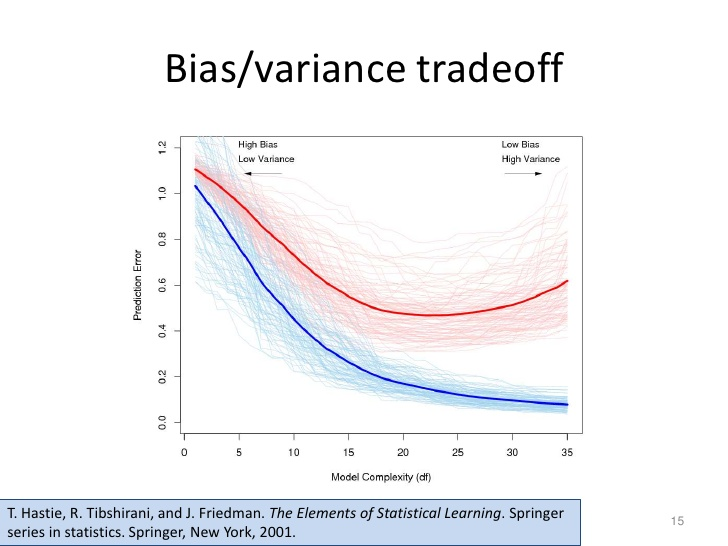
\includegraphics[width=1\textwidth]{art/support-vector-machine-15-728}
        \caption{Overfitting: 
        Prediction error on new data (red curve) versus the empirical prediction error (light blue).
        The empirical prediction error will always decrease as more complicated models are fit (moving right).
        The prediction error on new data, however, will not always decrease and will typically show a local minima.
        \label{fig:bias_variance}}
\end{figure}

Before we proceed, we now need to distinguish between several types of prediction errors.
The population \emph{risk} of a model parametrized by $\theta$, was previously defined as the average loss over all possible data instances, and denoted by $\risk(\theta)$ (\S \ref{sec:m_estimation}).
The empirical risk was defined as the average loss over the observed data points, and denoted by $\riskn(\theta)$.
We now update these definitions to deal with the the $\hyp(x)$ notation of the previous section.
\begin{align}
	\test :=& \expectg{Y,X}{\loss(Y,\hyp(X))}, \label{eq:test_error} \\
	\train :=& \expectn{\loss(y,\hyp(x))} = \frac{1}{n} \sum_i \loss(y_i,\hyp(x_i)),  \label{eq:training_error} \\
	\insample :=& \frac{1}{n} \sum_i \expectg{Y}{\loss(Y,\hyp(x_i))}, \label{eq:in_sample} \\
	\EPE :=& \expectg{\hat{\hyp}_n}{
		\expectg{Y,X}{\loss(Y,\hat{\hyp}_n(X))|\hat{\hyp}_n}
	}.\label{eq:epe}
\end{align}

Eq.(\ref{eq:test_error}) is merely a reformulation of $\risk(\theta)$ from Section~\ref{sec:m_estimation}.
It captures the expected loss, a given predictor, $\hyp(X)$, will incur on average when given new $X$'s and $Y$'s.
This will be the magnitude which will tell us which models perform well, and which do not.
It is known as the \emph{test error} or also as \emph{prediction error}.\marginnote{Test Error}

Eq.(\ref{eq:training_error}) is the reformulation of empirical risk, $\riskn(\theta)$, we have been optimizing in Section~\ref{sec:learning}.
We referred to it as the \emph{empirical risk}, but it is also known as the \emph{train error}.
\marginnote{Train Error}

Eq.(\ref{eq:in_sample}) is the average risk at the observed $x$'s, when given new $Y$'s \footnote{This magnitude should not be unfamiliar: e.g., inference in ANOVA is performed conditional on the $x$'s, which typically stem from a designed experiment.}.
This is the \emph{in sample error}.
\marginnote{In Sample Error}

Eq.(\ref{eq:epe}) is called the \emph{expected prediction error}, i.e., the expected loss when $\hyp$ is also re-learned. 
Put differently: How much would we err when:(1) we are given $n$ new examples $\sample_1$; (2) re-learn $\hat{\hyp}_n$ on $\sample_1$; (3) compute the risk of $\hat{\hyp}_n$ (in the population, not in $\sample_1$.
We emphasize this by writing $\hat{\hyp}_n$ instead of $\hyp$.
$\EPE$ is thus not a property of a particular predictor $\hyp$, but rather of a whole learning algorithm on random samples of size $n$.
It could have also been written as $\risk(algorithm)$, although I have not seen this notation in use.
\marginnote{Expected Prediction Error}


We would like to compare the performance of models based on $\test$, as this will give us an idea on the quality of the prediction on new data. 
Alas, computing $\test$ requires the distribution of $y$ and $x$, while we only have access to the $n$ observed samples.
Can the empirical risk $\train$ estimate the unknown risk $\test$? 
Figure~\ref{fig:bias_variance} suggests it cannot since $\train$ underestimates $\test$.
Why is this?
At an intuitive level: this is because with ERM we learn the $\hyp$ with smallest error in each sample.
It is thus the same as estimating the expected height in a population, by using the minimum in each sample; we will clearly be underestimating the expectation. Then again, there is the hope that we may take this minimum and debias it. 
This is the goal in the next sections.

Before proceeding, we distinguish between two similar tasks: 
\begin{description}
\item[Model Selection] This is the task of selecting between several candidate models.
\item[Model Assessment] This is the task of assessing the prediction error (i.e., the expected loss, the risk) of a given model.
\end{description}



\subsection{Train, Validate, Test}
\label{sec:train_test}
If data is abundant, a trivial, assumption free way to estimate $\test$\footnote{Think: why $\test$ is being estimated, and not $\EPE$ nor $\insample$?}, is to split the data into $3$ sets.
A \emph{training set}, used to learn several competing models.
A \emph{validation set}, used check the performance of the learned models and choose the best performer using some comparison measure. 
A \emph{test set}, used to estimate the risk, as the empirical risk $\train$ will be unbiased to the population risk $\test$.

If there is not enough data for this scheme, keep reading...


\subsection{Unbiased Estimators of the Risk}
\label{sec:risk_estimation}
Under appropriate assumptions, the bias in $\train$ when estimating $\insample$\footnote{In this case, note that it is $\insample$ being estimated, and not $\test$ nor $\EPE$.} can be computed analytically, and accounted for.
The bias $\insample-\train$ is called the \emph{optimism} of the algorithm.\marginnote{Optimism}
Akaike's Information Criterion (AIC), 
the finite sample Corrected AIC (AICc), 
Mallow's Cp (Cp), 
the Bayesian Information Criterion (BIC, aka SBC, aka SBIC), 
the Minimum Description Description Length (MDL), 
Vapnic's Structural Risk Minimization (SRM), 
the Deviance Information Criterion (DIC), 
and the Hannan-Quinn Information Criterion (HQC), 
all try to estimate $\insample$ by correcting for the optimism under different assumptions.\marginnote{Cp, AIC, BIC, MDL, SRM}

The differences, pros, and cons, of each will not be discussed herein. Just remember what they mean when you see them in your favourite software (R!).
They all have in common that you will want the model with the smallest criterion.
But be careful- as they are used for model selection, they are indifferent to scaling, and thus should be not interpreted as the expected prediction error.

\begin{remark}
Not all model selection criteria estimate $\insample$. The Focused Information Criterion (FIC), for example, does not.
\end{remark}





\paragraph{Further Reading}
For a brief review of AIC, BIC, MDL and SRM see Chapter 7 in \citep{hastie_elements_2003}. 
For a more rigorous derivation, see \cite{claeskens_model_2008}.





\subsection{Jackknifing}
\label{sec:jackknife}

If concerned with over fitting, here is a simple algorithm to estimate the prediction error:

\begin{algorithm}[H]
\caption{Jackknife}
\begin{algorithmic}
\For {$i \in 1,\dots,n$}
    \State $\hat{\hyp}^{(i)} \gets$ the learned model with all but the $i$'th observation.
    \State $\loss^{(i)} \gets$ the loss of $\hat{\hyp}^{(i)}$ on the $i$'th observation.
\EndFor
\State \Return the average loss over $\loss^{(i)}$.
\end{algorithmic}
\end{algorithm}

This process is called the \emph{Jackknife}, or \emph{Leave-One-Out--Cross-Validation}. 
This algorithm return an estimator of $\EPE$.
This might be quite surprising: every split uses almost an identical sample, so why would it not estimate $\test$? See Section 7.12 in \cite{hastie_elements_2003} for details..

But wait! We might be able to stabilize the variability of the estimated error in every split, if instead of leaving only a single observation aside, we leave some more. This lead to way to \emph{K-Fold Cross Validation} in the next section.


\subsection{Cross Validation}
\label{sec:cv}

\begin{algorithm}[H]
\caption{Cross Validation}
\begin{algorithmic}
\State Split the data into $\folds$ parts (``folds'').
\For {$\fold \in 1,\dots,\folds$}
    \State $\hat{\hyp}^{(k)} \gets$ the learned model with all \emph{except} the observations in the $\fold$'th fold.
    \State $\loss^{(\fold)} \gets$ the loss average of $\hat{\hyp}^{(\fold)}$ on the observations in the $\fold$'th fold.
\EndFor
\State \Return the average over $\loss^{(\fold)}$ .
\end{algorithmic}
\end{algorithm}

This simple algorithm estimates $\EPE$ without any assumption on the data generating process, and less data than would be required for a ``train-validate-test'' scheme.
Well, as it actually serves for model selection, it should be seen as a ``train-validate'' scheme, without the ``test'' part. It is thus \emph{not} an unbiased estimate of $\EPE$. See Section 7.12 in \cite{hastie_elements_2003} for details.

But wait again! 
The Cross Validation scheme resamples the data \emph{without replacement} to estimate $\EPE$. Could we have sampled it \emph{with} replacement? Yes. This is the idea underlying the \emph{Bootstrapping} scheme.


\subsection{Bootstrapping}
\label{sec:bootstrap}

Here is the simplest version of Bootstrap validation:

\begin{algorithm}[H]
\caption{Bootstrap}
\begin{algorithmic}
\For {$\bootstrap \in 1,\dots,\bootstraps$}
	\State $\sample^\bootstrap \gets$ $n$ randomly selected observations, with replacement, from the original data.
    \State $\hat{\hyp}^{\bootstrap} \gets$ the model learned with  $\sample^\bootstrap$.
    \State $\loss^{\bootstrap} \gets$ the average loss of $\hat{\hyp}^{\bootstrap}$ on the observations in the \emph{original} data.
\EndFor
\State \Return the over of $\loss^{\bootstrap}$ .
\end{algorithmic}
\end{algorithm}

This algorithm is not a good estimator of $\EPE$ as observations play a role both in learning and in validating. 
Several corrections are available. For details see Section 7.11 in \cite{hastie_elements_2003}.

The Bootstrap is a very general scheme, which can be used not only for model validation, but for assessing many of its statistical properties. It is possibly best known when used for hypothesis testing. 
For more on the Bootstrap, see \cite{efron_introduction_1994}.






%%%%%%%%% Unsupervised %%%%%%%%%%%

\section{Unsupervised Learning}
\label{sec:unsupervised}

Unlike Supervised Learning, in Unsupervised Learning there is not outcome variable. There is thus no notion of ``right'' and ``wrong''. 
We merely want to learn the joint distribution of the data, $X \in \featureS$, and represent it in some way we can understand. 
Well, maybe ``merely'' is not the right word, as learning the joint distribution of the data means that instead of learning the relation between a set $x$ and another, $y$, we now try to learn the relation between all pairs of variables in $x$, which is clearly more challenging. 

Describing the data via it's joint distribution is the pinnacle, but would require many samples if $x$ has a high dimension (by high we mean $p>3$!). For higher dimensions we need to set more modest goals.

The different goals of unsupervised learning are
\begin{description}
\item[Density Estimation] Estimate the joint density of $x$ over $\featureS$.
\item[Detect high density regions] Find feature combinations which tend to concentrate, hopefully, because the belong to homogenous and interpretable subgroups.
\item[Find low dimensional representations] Find a low dimensional representation of the joint distribution. This allows the learning from realistic sample sizes, and analysis by, e.g., interpretable parameters and visualization.
This goal is discussed in Section~\ref{sec:dim_reduce}.
\end{description}


\paragraph{Relation to Supervised Classification}
Any supervised classification problem can be solved, at least in theory, by solving an unsupervised. 
I.e., estimate the joint distribution within each class, and then classify new observations to the highest density class, via Bayes rule. 
This is known as a \emph{generative} model, as we try to learn the full data generating distribution, unlike the \emph{discriminative} models described above, where the distribution of the features $x$ is of no interest.





\subsection{Density Estimation}
\label{sec:density_estimation}

\subsubsection{Parametric Density Estimation}
Density estimation deals with the learning of the data generating distribution.
If a parametric generative model can be assumed, this collapses to an unsupervised ERM problem. 
Maximum Likelihood estimation being a particularly attractive approach.
If a parametric model cannot be assumed, we fall into the real of non-parametric methods. As we saw for Supervised learning, these typically rely on pooling information from neighbourhoods of $\featureS$.

\subsubsection{Kernel Density Estimation}

Much like the Kernel Smoothing regression, a \naive estimator is the moving average.
A natural generalization, in the spirit of the Nadaraya-Watson smoother (Eq.(\ref{eq:nadaraya_watson})) is the \emph{Parzen} estimate:\marginnote{Parzen Estimate}
\begin{align}
\label{eq:parzen}
	\hat{\pdf}(x):=\frac{1}{n \lambda} \sum_{i=1}^n \kernel_\lambda(x,x_i).
\end{align}

\begin{remark}
If you have been convinced by the use of KNN (\S\ref{sec:knn}) for regression (or classification), there is no reason not to use it for density estimation. It will keep offering the same pros and cons as in KNN regression (or classification).
\end{remark}

As previously stated, these methods may fail when $x$ are high dimensional. We thus recur to other methods.


\subsection{Detect High Density Regions}
When data data is high dimensional so that we cannot perform density estimation, or when we are merely interested in grouping observations, we can still detect high density regions where observations ``clump'' together. Hopefully, into meaningful homogenous groups.
These groups are called \emph{clusters}, thus these methods are known as \emph{cluster analysis}, or \emph{data segmentation} methods.\marginnote{Cluster Analysis, Data Segmentation}

Since these methods are aim at detecting data clustering, they clearly imply the availability of some measure of distance, or similarity, between data points. 


\subsubsection{K Means Clustering}
\label{sec:kmeans}
The idea behind K-means clustering is to find a representative point for each of K clusters, and assign each (unlabeled) data point to one of these clusters. As each cluster has a representative point, this is also a \emph{prototype method}.\marginnote{Prototype Methods}.
The clusters are defined so that they minimize the average distance between all points to the center of the cluster.

In K-means, the clusters are first defined, and then similarities computed. This is thus a \emph{top-down} method.\marginnote{Top Down Clustering}

\begin{algorithm}[H]
\caption{K-Means}
\begin{algorithmic}
\State Choose the number of clusters $K$.
\State Arbitrarily assign points to clusters.
\While {Clusters keep changing}
	\State Compute the cluster centers as the average of their points.
	\State Assign each point to its closest cluster center (in Euclidean distance).
\EndWhile
\State \Return Cluster assignments and means.
\end{algorithmic}
\end{algorithm}



\paragraph{K-Medoids}
If a Euclidean distance is inappropriate for a particular $\featureS$, or that robustness to corrupt observations is required, or that we wish to constrain the cluster centers to be actual observations, then the \emph{K-Medoids} algorithm is an adaptation of K-means that allows this.

\begin{algorithm}[H]
\caption{K-Medoids}
\begin{algorithmic}
\State Choose a similarity metric $\similarity(x_i,x_j)$.
\State Choose the number of clusters $K$.
\State Arbitrarily assign points to clusters.
\While {Clusters keep changing}
	\State Within each cluster, set the center as the data point that minimizes the sum of distances to other points in the cluster.
	\State Assign each point to its closest cluster center (in $\similarity(x_i,x_j)$ distance).
\EndWhile
\State \Return Cluster assignments and centers.
\end{algorithmic}
\end{algorithm}


See Section 14.3.10 in \cite{hastie_elements_2003}.


\subsubsection{Hierarchical Clustering}
\label{sec:hierarchical}
[TODO]



\subsubsection{Association Rules}
\label{sec:association}
[TODO]


% Generative models %

\section{Generative Models}
For the mere purpose of making a prediction, we do not need to learn the full data generating distribution $\dist(y,x)$. 
Knowing this distribution, however, does permit to make predictions, via Bayes Theorem: 
$\dist(y|x)=\frac{\dist(y,x)}{\int\dist(y,x)dy}$.
Several supervised and unsupervised methods make use of this relation to make predictions. These are known as \emph{generative models} .
Since the generative distribution serves both in supervised and unsupervised learning, we have dedicated it a section of its own.

\subsection{Density Estimation}
Clearly, the trivial generative model is the density estimation, discussed in Section~\ref{sec:density_estimation}.


\subsection{Fisher's Linear Discriminant Analysis (LDA)}
\label{sec:lda}
The fundamental idea behind Fisher's LDA (sometimes, just LDA) is that for dichotomous $y$'s: $\dist(x|y)$ is multivariate Gaussian, with the same covariance for all $y$.
Estimating $\dist(x|y)$ thus amounts to the estimation of the mean and covariance, which are fairly simple problems that do not require too much data (relatively).

The decision boundaries of this method turn out to be linear in $\featureS$. 
Denoting the distance from the class centers by $\hat{\delta}:=(\hat{\mu}_1-\hat{\mu}_2)$, class thus 2 will be predicted if 
\begin{align}
	x' \hat{\Sigma}^{-1} \hat{\delta} > \frac{1}{2} \hat{\delta}' \hat{\Sigma}^{-1} \hat{\delta}
\end{align}
and class 1 otherwise.


\paragraph{Relation to OLS classification}
Interestingly, the two-class LDA, is the same as a regression classifier from  Section~\ref{sec:regression_classifier} \cite[Eq. 4.11 ]{hastie_elements_2003}.



\subsection{Fisher's Quadratic Discriminant Analysis (QDA)}
If you are uncomfortable with the fixed covariance assumption of LDA, one can relax thus assumption.
This leads to QDA, which is more flexible than LDA, requiring slightly more data, but permitting the learning of a class of quadratic classifiers, and not only linear.






\subsection{\Naive Bayes}
\label{sec:naive_bayes}
In LDA we dealt with the problem of estimating high dimensional distributions by adding the class-wise Gaussianity assumption. As Gaussians as fairly simple to learn from data, if there is any truth to this assumption, our life improved. 
Another life-simplifying assumption, replacing the Gaussianity assumption, is that $\dist(x|y)$ is the product of the margins, i.e., the the features are independent within each class: $\dist(x|y)=\prod_{j=1}^p\dist(x_j|y)$
This greatly simplifies things as estimating the univariate marginal distributions $\dist(x_j|y)$ is a fairly simple problem, which can be done non-parametrically by Kernel smoothing for continuous predictors (\S\ref{sec:kernel}), and simple relative frequencies for discrete predictors. 


%%%%%%%%% Dimension Reduction %%%%%%%%%%%
\section{Dimensionality Reduction}
\label{sec:dim_reduce}
[TODO]

\subsection{Dimensionality Reduction In Supervised Learning}
[TODO]


\subsubsection{Model Selection}
[TODO]
%\cite{foster_variable_2004}

\subsubsection{LASSO}
[TODO]


\subsection{Dimensionality Reduction in Unsupervised Learning}
[TODO]


\subsubsection{PCA}
[TODO]

\subsubsection{Multidimensional Scaling (MDS)}
[TODO]


\subsubsection{Self Organizing Maps}
[TODO]


\subsubsection{Principal Curves}
[TODO]

\subsubsection{ICA}
[TODO]

\subsubsection{kPCA}
[TODO]

\subsubsection{ISOmap}
[TODO]


\subsubsection{LLE}
[TODO]



%%%%%%%%% Latent Space Models%%%%%%%%%%%
\section{Latent Space Models}
\label{sec:latent_space}
[TODO]


\subsection{Mixtures}
[TODO]


\subsection{Regression Switching}
[TODO]



\subsection{Factor Analysis}
[TODO]


\subsection{Hidden Markov}
[TODO]


\subsection{Collaborative Filtering}
[TODO]







%%%%%%%%% Algorithms %%%%%%%%%%%
\newpage
\listofalgorithms


%%%%%%%%% Bibliography %%%%%%%%%%%
\bibliographystyle{abbrvnat}
\bibliography{Intro2MachineLearning}


\end{document}